% =====================================================================
%  TuniBot -- CSTAM 3.0 Challenge -- Technical Report (Phases 1 to 3)
%  Team ConnectENIT
%  Compile: pdflatex main.tex (twice), or upload the folder to Overleaf.
%  The figures/ folder must sit next to this file. Missing Gazebo/RViz
%  screenshots are replaced by a placeholder box, so it always compiles.
% =====================================================================
\documentclass[11pt,a4paper]{article}

\usepackage[utf8]{inputenc}
\usepackage[T1]{fontenc}
\usepackage[english]{babel}
\usepackage{lmodern}
\usepackage{microtype}
\usepackage[margin=2.3cm]{geometry}
\usepackage{amsmath,amssymb}
\usepackage{graphicx}
\usepackage{float}
\usepackage{caption}
\usepackage{subcaption}
\usepackage{booktabs}
\usepackage{tabularx}
\usepackage{array}
\usepackage{enumitem}
\usepackage{xcolor}
\usepackage{tikz}
\usetikzlibrary{arrows.meta,positioning,fit,backgrounds,calc}
\usepackage{fancyhdr}
\usepackage{titlesec}
\usepackage{xurl}
\usepackage[hidelinks]{hyperref}

% ---------- Colours (taken from the web interface) ----------
\definecolor{copper}{HTML}{1D6B4F}
\definecolor{ochre}{HTML}{F0B23A}
\definecolor{manganese}{HTML}{2B1D19}
\definecolor{chili}{HTML}{C2412D}
\definecolor{slip}{HTML}{F3F7F2}

\hypersetup{colorlinks=true,linkcolor=copper,urlcolor=copper,citecolor=copper}
\titleformat{\section}{\Large\bfseries\color{manganese}}{\thesection}{0.6em}{}
\titleformat{\subsection}{\large\bfseries\color{copper}}{\thesubsection}{0.6em}{}
\titleformat{\subsubsection}{\normalsize\bfseries\color{manganese}}{\thesubsubsection}{0.6em}{}
\setlist{itemsep=2pt,topsep=4pt}
\newcolumntype{L}{>{\raggedright\arraybackslash}X}

\pagestyle{fancy}
\fancyhf{}
\lhead{\small TuniBot -- Technical Report}
\rhead{\small CSTAM 3.0 -- Team ConnectENIT}
\cfoot{\thepage}

% Include a screenshot if it exists, otherwise draw a labelled placeholder.
\newcommand{\shot}[2]{%
  \IfFileExists{figures/#2}{\includegraphics[width=#1]{figures/#2}}{%
    \fbox{\parbox[c][4cm][c]{\dimexpr#1-2\fboxsep-2\fboxrule\relax}{\centering\small\color{chili}Screenshot to add:\\\texttt{figures/\detokenize{#2}}}}}}

\begin{document}

% =====================================================================
\begin{titlepage}
  \centering
  \vspace*{1.5cm}
  {\large CSTAM 3.0 -- TuniBot Challenge\par}
  \vspace{0.6cm}
  {\color{copper}\rule{\linewidth}{1.2pt}\par}
  \vspace{0.5cm}
  {\Huge\bfseries\color{manganese} TuniBot\par}
  \vspace{0.3cm}
  {\LARGE Autonomous Service Robot for Indoor Delivery\par}
  \vspace{0.3cm}
  {\Large Technical Report -- Phases 1, 2 and 3\par}
  {\color{copper}\rule{\linewidth}{1.2pt}\par}
  \vspace{1.2cm}
  {\Large\bfseries Team ConnectENIT\par}
  \vspace{0.2cm}
  {\large Wassim Toukebri \quad Maram Hammami \quad Ridha Charrad\par}
  \vspace{0.2cm}
  {\normalsize IEEE ENIT Computer Society Student Branch Chapter\par}
  \vspace{1.2cm}
  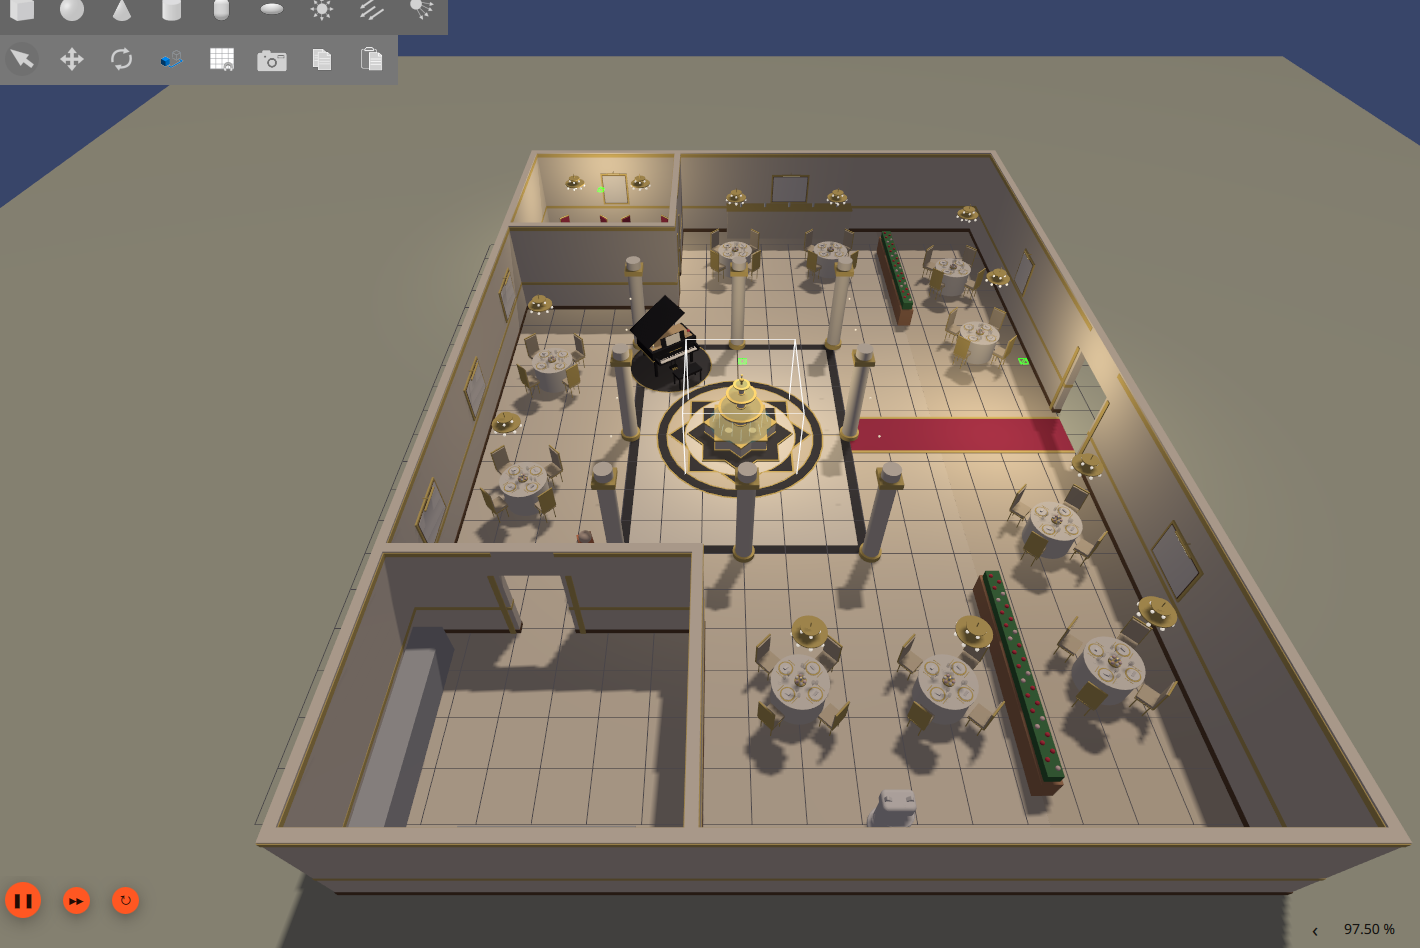
\includegraphics[width=0.78\linewidth]{figures/gz_restaurant.png}\par
  \vfill
  {\large \today\par}
  \vspace{0.3cm}
  {\small Repository: \url{https://github.com/maramhammami-svg/tunibot-phase3}\par}
\end{titlepage}

\tableofcontents
\newpage

% =====================================================================
\section*{Abstract}
\addcontentsline{toc}{section}{Abstract}

TuniBot is a complete ROS~2 software stack for an autonomous waiter robot
that serves a restaurant from the guest's order to the robot's return to
its charger, with no human in the loop. It runs on ROS~2 Jazzy, Gazebo
Harmonic and Nav2, on a simulated BellaBot differential-drive robot with a
2D LiDAR, in two restaurant worlds: an open lounge with 24 tables and
\emph{Dar Tunibot}, a traditional Tunisian restaurant with 1.20\,m arched
doorways.

The project was built in three phases. \textbf{Phase~1} delivers the
foundations: SLAM mapping, AMCL localization, Nav2 navigation to every
table, a delivery task queue with editing, cancellation and preemption,
and automatic return to the dock. \textbf{Phase~2} makes the robot robust:
a walking pedestrian that the robot detects and plans around, costmaps
tuned for narrow doorways with a multi-stage recovery, and a physical
24\,V Li-ion battery model with a low and critical return-to-dock policy.
\textbf{Phase~3} adds the user layer: a web Client page where guests pick
their table on the floor plan and order by tapping or by voice (French,
English and Tunisian Darija), and an Admin control room where staff watch
the robot, its battery and its queue live. Voice command integration for
placing orders is our bonus functionality. The web layer is a separate
ROS~2 package that only uses existing topics.

The system is covered by 65 automated tests (9 Phase~1 unit tests,
5 Phase~2 integration tests and 51 web tests), all passing, and by
end-to-end runs in Gazebo where a web order was delivered to its table.

% =====================================================================
\section{Team Overview and Contributions}

We are \textbf{ConnectENIT}, a team of three students from the IEEE ENIT
Computer Society Student Branch Chapter. All three of us worked on every
phase of the challenge: we designed, coded, tested and reviewed together.
To move fast, each member led one area in each phase while the others
reviewed and tested it, as summarised in Table~\ref{tab:team}.

\begin{table}[H]
\centering
\small
\begin{tabularx}{\linewidth}{l L L L}
\toprule
\textbf{Member} & \textbf{Phase 1: Foundations} & \textbf{Phase 2: Integration} & \textbf{Phase 3: UI/UX \& docs} \\
\midrule
Wassim Toukebri & Nav2 navigation set-up, waypoints to tables & Dynamic obstacle avoidance, costmap tuning for narrow doorways, recovery behaviours & FastAPI server and ROS~2 bridge, order tracking, Gazebo validation \\
\addlinespace
Maram Hammami & Delivery task queue manager and auto-docking & Battery model and return-to-dock policy, Dar Tunibot world & Client page UX and visual design, voice ordering (French, English, Darija), technical report \\
\addlinespace
Ridha Charrad & Gazebo world and robot model, SLAM mapping, AMCL localization & Integration tests, pedestrian scenarios & Admin control room, automated tests, demo video \\
\bottomrule
\end{tabularx}
\caption{Each member's lead area per phase. All members contributed to all three phases.}
\label{tab:team}
\end{table}

% =====================================================================
\section{Problem Statement and Industrial Context}

Restaurant service still depends on staff walking every plate and drink
from the kitchen to the table. That repetitive work takes time away from
guests, and it scales badly at peak hours. Service robots such as the
BellaBot are now common in Asian restaurants, but they need software that
copes with real venues: narrow aisles, people walking around, a battery
that runs out and guests who want to know where their order is.

The CSTAM~3.0 challenge, set with our industrial partner TuniBot, a
Tunisian robotics and automation company, asks for a software-only answer
built in three phases. The robot must:
\begin{itemize}
  \item map an indoor environment and localize itself in it;
  \item receive food and beverage requests and queue them;
  \item drive autonomously to predefined tables to deliver them, safely around furniture and people;
  \item return to its dock to charge when idle or low on battery;
  \item handle narrow passages and moving obstacles, and recover when blocked (Phase~2);
  \item give guests an interface to order and staff an interface to supervise the robot (Phase~3).
\end{itemize}

Two constraints shaped the design. Everything runs in simulation with
industry-standard open-source tools (ROS~2, Gazebo, Nav2), so the stack
can move to a real robot later. And the result must work in a realistic
venue: besides a large lounge, we built Dar Tunibot, a traditional
Tunisian restaurant whose 1.20\,m arched doorways and narrow aisles are a
hard case for any navigation stack.

% =====================================================================
\section{Proposed Solution}

Our solution is a layered ROS~2 system: a simulated restaurant and robot at
the bottom, the robot's core logic in the middle and a web interface on
top. Each layer talks to the next only through ROS~2 topics and actions,
so each can be tested and replaced on its own.

\begin{table}[H]
\centering
\begin{tabularx}{\linewidth}{l L c}
\toprule
\textbf{Layer} & \textbf{What it does} & \textbf{Phase} \\
\midrule
Simulation & Gazebo Harmonic worlds (Restaurant Lounge, 24 tables; Dar Tunibot, 10 tables), BellaBot differential-drive model with 2D LiDAR and wheel odometry, a walking pedestrian & 1, 2 \\
Mapping and localization & SLAM Toolbox to build the maps, AMCL to localize, auto-initialized at the dock & 1 \\
Navigation & Nav2: NavFn global planner, DWB local controller, behaviour tree and recoveries; costmaps tuned for 1.20\,m doorways & 1, 2 \\
Delivery task manager & FIFO queue of delivery requests, dispatch to tables, modify and delete, preemption, recovery that keeps the order queued & 1, 2 \\
Auto-docking & Return to dock when idle, docking sequence, rest and charge & 1 \\
Dynamic obstacles & Pedestrian controller (patrol, cross, block, clear); 10\,Hz local costmap so Nav2 re-plans around people & 2 \\
Battery & 24\,V 20\,Ah Li-ion NMC model with voltage sag and temperature; return to dock at 25\,\%, emergency dock at 15\,\%, recharge to 80\,\% & 2 \\
Operator tools & Mission Control simulator (Tkinter GUI and CLI) for dispatching and testing & 1, 2 \\
Web interface & Client ordering page with voice orders, Admin control room, FastAPI bridge to ROS~2 & 3 \\
\bottomrule
\end{tabularx}
\caption{Layers of the TuniBot software stack.}
\end{table}

\subsection{Requirements coverage}

\begin{table}[H]
\centering
\small
\begin{tabularx}{\linewidth}{c l L}
\toprule
\textbf{Phase} & \textbf{Requirement} & \textbf{How we met it} \\
\midrule
1 & Simulated environment & Two Gazebo worlds with tables, kitchen and dock; BellaBot model with LiDAR and odometry \\
1 & Mapping and localization & SLAM Toolbox maps of both worlds; AMCL localization initialized at the dock \\
1 & Autonomous navigation & Nav2 goals to 24 + 10 predefined table waypoints, kitchen and dock \\
1 & Delivery task management & FIFO queue with live edit, delete, cancel and preemption of docking by a new order \\
1 & Auto-docking & Return to dock after an idle timeout or on command; stop docking at any time \\
\midrule
2 & Dynamic obstacle avoidance & Pedestrian in four modes; fast local costmap so Nav2 re-plans around the person \\
2 & Complex layout handling & Inflation tuned for 1.20\,m doorways; reverse, clear and re-plan recovery, up to 3 retries \\
2 & Battery and state simulation & Physical Li-ion model; 25\,\% / 15\,\% / 80\,\% docking policy \\
\midrule
3 & Ordering interface (web or mobile) & Responsive Client page: table on the floor plan, menu book, voice ordering, live tracking, several orders \\
3 & Admin view: robot status and battery & Admin control room: live map with Nav2 path, mission, battery, queue, health, log, controls \\
3 & Documentation & This report, the repository README and the demonstration video \\
\bottomrule
\end{tabularx}
\caption{Challenge requirements and how they are met.}
\end{table}

% =====================================================================
\section{System Design}

\subsection{Architecture}

Figure~\ref{fig:arch} shows the whole system. The Phase~1 and Phase~2
nodes form the robot; the Phase~3 web package sits on top and reaches the
robot only through the topics the other nodes already use.

\begin{figure}[tbp]
\centering
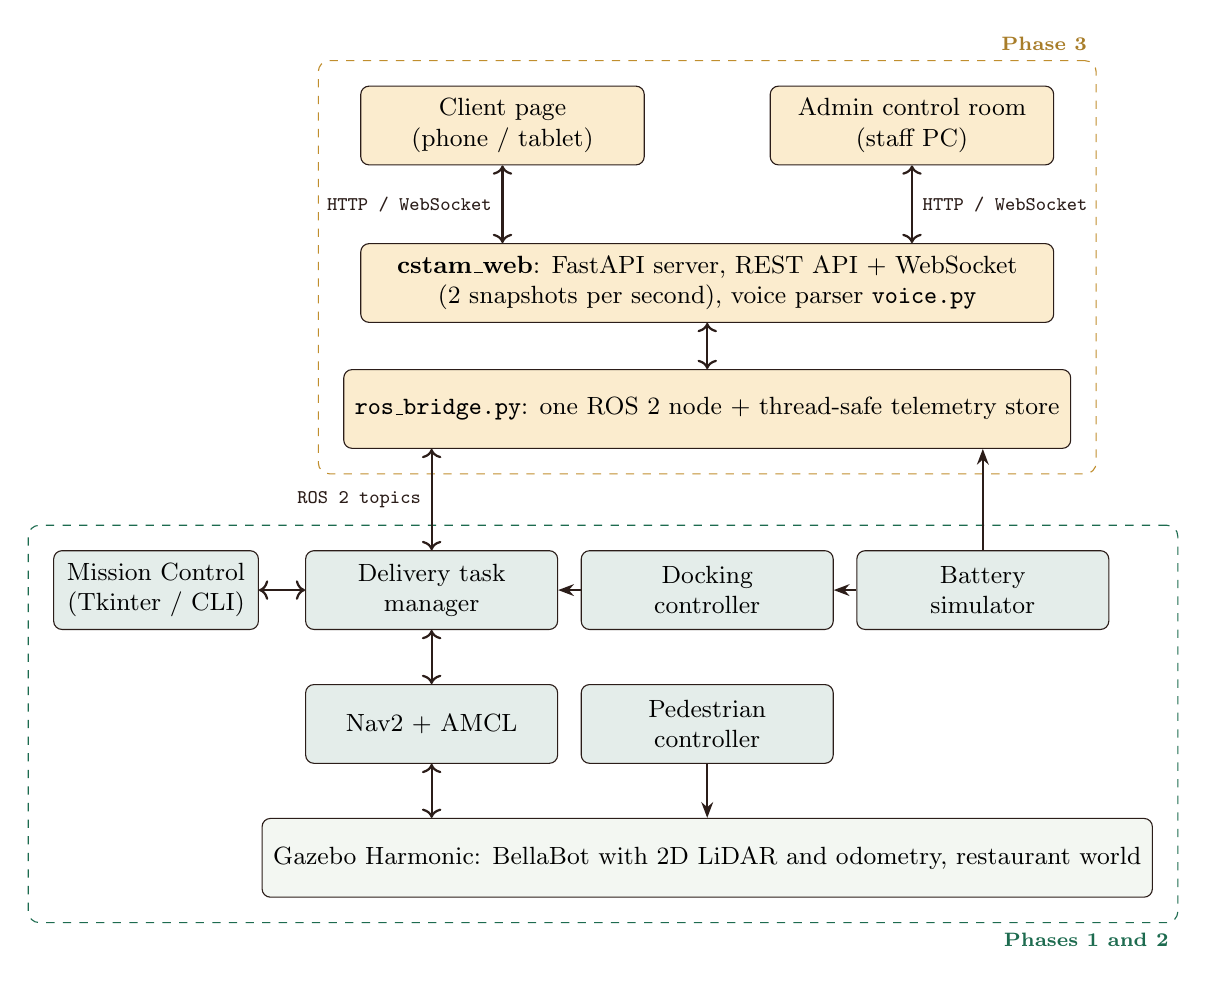
\begin{tikzpicture}[
  box/.style={draw=manganese,rounded corners=3pt,align=center,
              minimum height=1.0cm,font=\small,inner sep=4pt},
  web/.style={box,fill=ochre!25},
  ros/.style={box,fill=copper!12,minimum width=3.2cm},
  sim/.style={box,fill=slip},
  arr/.style={-{Stealth[length=2mm]},thick,manganese},
  lab/.style={font=\scriptsize\ttfamily,fill=white,inner sep=1.5pt}
]
% Phase 3
\node[web,minimum width=3.6cm] (client) at (-2.6,0) {Client page\\(phone / tablet)};
\node[web,minimum width=3.6cm] (admin)  at ( 2.6,0) {Admin control room\\(staff PC)};
\node[web,minimum width=8.8cm] (server) at (0,-2.0) {\textbf{cstam\_web}: FastAPI server, REST API + WebSocket\\(2 snapshots per second), voice parser \texttt{voice.py}};
\node[web,minimum width=8.8cm] (bridge) at (0,-3.6) {\texttt{ros\_bridge.py}: one ROS~2 node + thread-safe telemetry store};
% Phases 1-2
\node[ros] (tm)   at (-3.5,-5.9) {Delivery task\\manager};
\node[ros] (dock) at ( 0,  -5.9) {Docking\\controller};
\node[ros] (bat)  at ( 3.5,-5.9) {Battery\\simulator};
\node[ros] (nav)  at (-3.5,-7.6) {Nav2 + AMCL};
\node[ros] (ped)  at ( 0,  -7.6) {Pedestrian\\controller};
\node[ros,minimum width=2.6cm] (mc) at (-7.0,-5.9) {Mission Control\\(Tkinter / CLI)};
\node[sim,minimum width=10.2cm] (gz) at (0,-9.3) {Gazebo Harmonic: BellaBot with 2D LiDAR and odometry, restaurant world};

\draw[arr,<->] (client.south) -- node[lab,left=2pt]{HTTP / WebSocket} (client.south |- server.north);
\draw[arr,<->] (admin.south)  -- node[lab,right=2pt]{HTTP / WebSocket} (admin.south |- server.north);
\draw[arr,<->] (server) -- (bridge);
\draw[arr,<->] (bridge.south -| tm) -- node[lab,left=2pt]{ROS 2 topics} (tm.north);
\draw[arr] (bat.north) -- (bridge.south -| bat);
\draw[arr] (dock) -- (tm);
\draw[arr] (bat) -- (dock);
\draw[arr,<->] (tm) -- (nav);
\draw[arr,<->] (mc) -- (tm);
\draw[arr,<->] (nav) -- (nav |- gz.north);
\draw[arr] (ped) -- (ped |- gz.north);

\begin{scope}[on background layer]
  \node[draw=ochre!80!black,dashed,rounded corners,fit=(client)(admin)(server)(bridge),inner sep=9pt] (p3) {};
  \node[anchor=south east,font=\scriptsize\bfseries,text=ochre!70!black] at (p3.north east) {Phase 3};
  \node[draw=copper,dashed,rounded corners,fit=(tm)(bat)(nav)(mc)(gz),inner sep=9pt] (p12) {};
  \node[anchor=north east,font=\scriptsize\bfseries,text=copper] at (p12.south east) {Phases 1 and 2};
\end{scope}
\end{tikzpicture}
\caption{System architecture. Arrows are ROS~2 topics or actions, except HTTP / WebSocket between the browsers and the web server.}
\label{fig:arch}
\end{figure}

The workspace has four ROS~2 packages:
\begin{itemize}
  \item \texttt{cstam\_gazebo}: worlds, BellaBot and pedestrian models, Gazebo--ROS bridge (Phases 1--2);
  \item \texttt{cstam\_navigation}: Nav2, AMCL and SLAM parameters, maps, table waypoints, launch files (Phases 1--2);
  \item \texttt{cstam\_core}: task manager, docking controller, battery simulator, pedestrian controller (Phases 1--2);
  \item \texttt{cstam\_web}: web server, ROS~2 bridge and the Client and Admin pages (Phase~3).
\end{itemize}

\subsection{Simulation environment}

\IfFileExists{figures/gz_resto_arbi.png}{%
\begin{figure}[H]
\centering
\begin{subfigure}[t]{0.49\linewidth}\centering
  \includegraphics[width=\linewidth]{figures/gz_resto_arbi.png}
  \caption{Dar Tunibot (10 tables, 1.20\,m arches).}
\end{subfigure}\hfill
\begin{subfigure}[t]{0.49\linewidth}\centering
  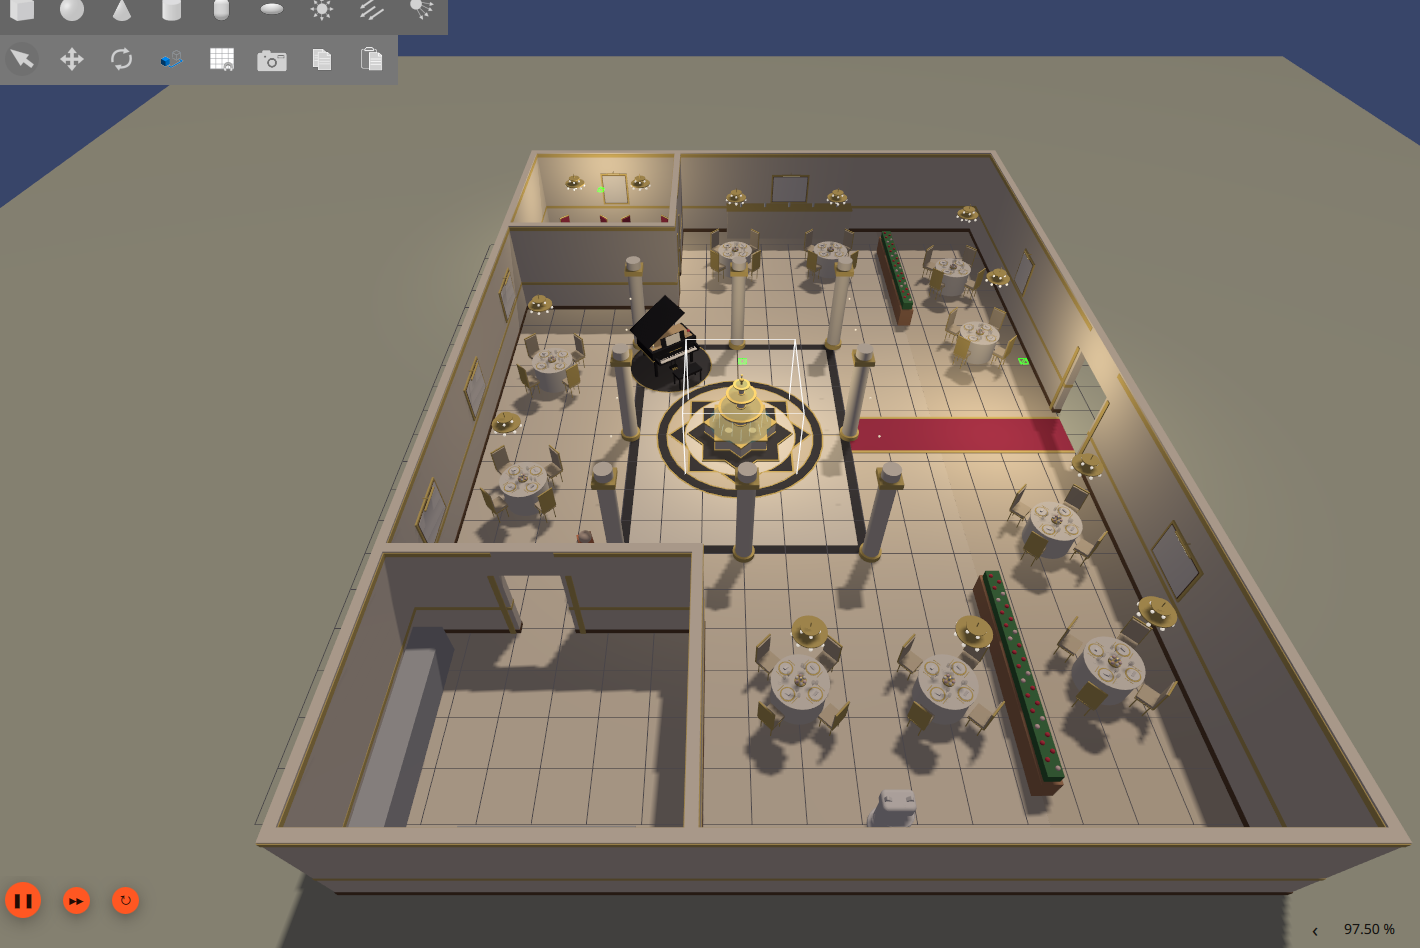
\includegraphics[width=\linewidth]{figures/gz_restaurant.png}
  \caption{Restaurant Lounge (24 tables).}
\end{subfigure}
\caption{The two restaurant worlds in Gazebo Harmonic.}
\end{figure}}{%
\begin{figure}[H]
\centering
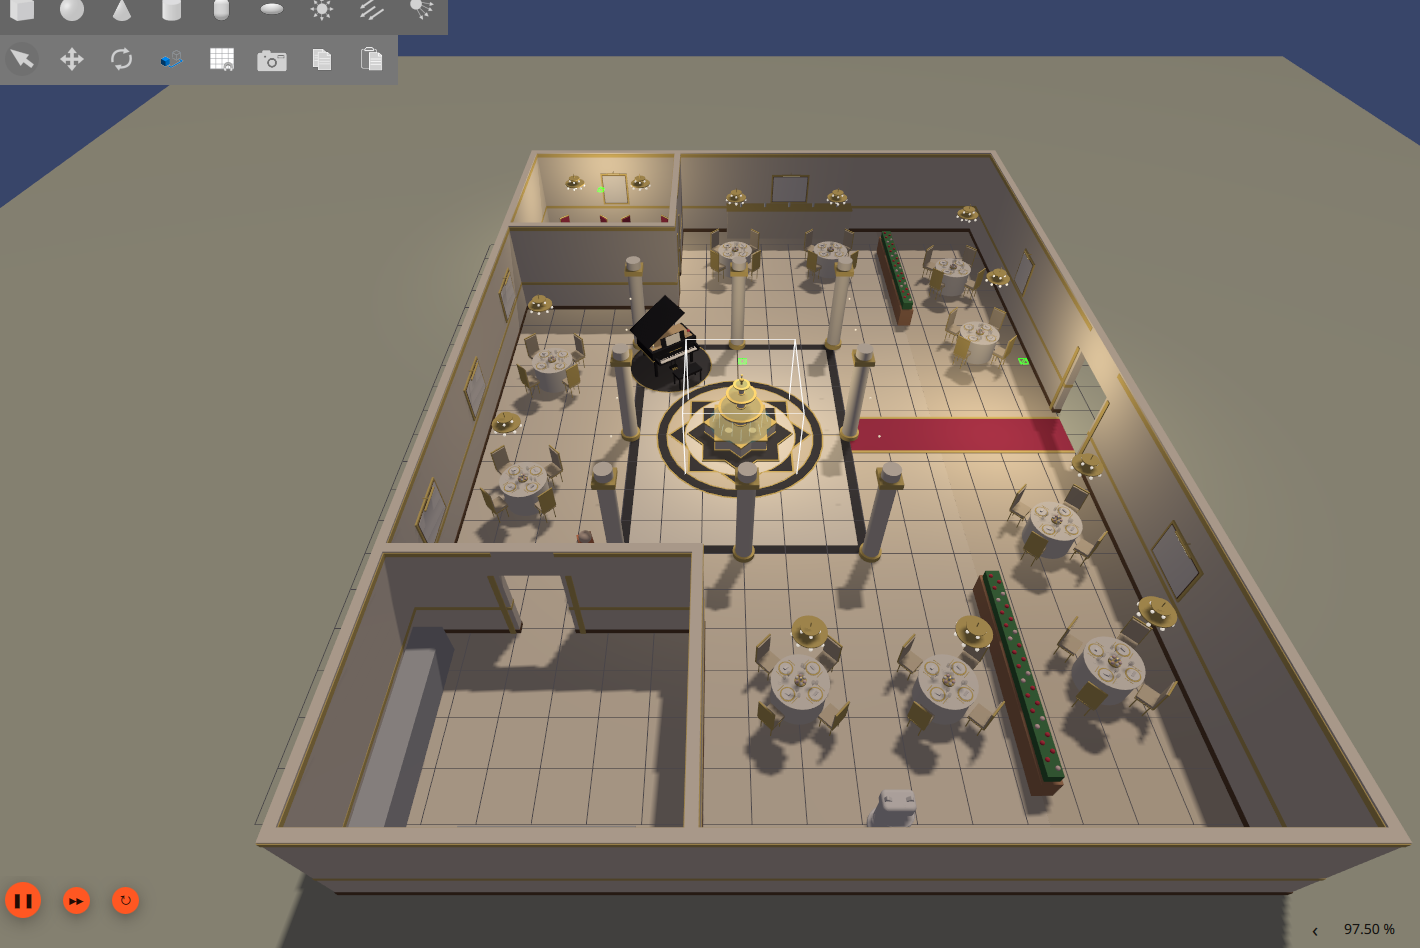
\includegraphics[width=0.75\linewidth]{figures/gz_restaurant.png}
\caption{The Restaurant Lounge world in Gazebo Harmonic (24 tables, kitchen counter and dock).}
\end{figure}}

\begin{itemize}
  \item \textbf{Restaurant Lounge} (\texttt{restaurant.world}): 24 tables in four rows, a kitchen pickup counter on the west side and a resting dock in the south-east corner at $(7.06, -12.00)$.
  \item \textbf{Dar Tunibot} (\texttt{resto\_arbi.world}): a traditional Tunisian house with a central fountain, a north-wing kitchen, 10 tables, a dock on the west wall and 1.20\,m stone arch doorways.
  \item \textbf{BellaBot}: a differential-drive base (radius 0.28\,m, top speed 0.45\,m/s) with a 2D LiDAR at $z\approx0.2$\,m and wheel odometry, bridged to ROS~2 (\texttt{/scan}, \texttt{/odom}, \texttt{/cmd\_vel}).
  \item \textbf{Pedestrian}: a 1.70\,m human model on a hidden differential-drive chassis, so it stays upright and is seen by the LiDAR (see Section~\ref{sec:issues}).
\end{itemize}

\subsection{Mapping and localization}

We built one occupancy-grid map per world with SLAM Toolbox, driving the
robot through the restaurant (\texttt{run\_mapping\_demo.sh}) and saving
the result with \texttt{save\_map.sh} (Figure~\ref{fig:maps}). At run time
the robot localizes on that map with AMCL. Its initial pose is published
automatically at the dock, so the robot is localized as soon as the
system starts, with no manual ``2D Pose Estimate''.

\begin{figure}[H]
\centering
\begin{subfigure}[t]{0.44\linewidth}\centering
  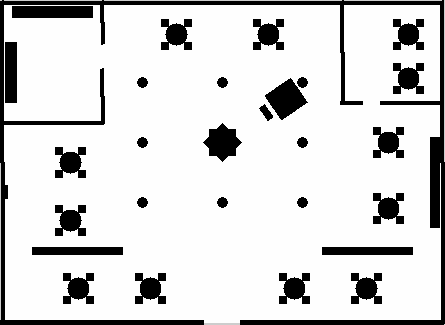
\includegraphics[width=\linewidth]{figures/resto_arbi_map.png}
  \caption{Dar Tunibot.}
\end{subfigure}\hfill
\begin{subfigure}[t]{0.50\linewidth}\centering
  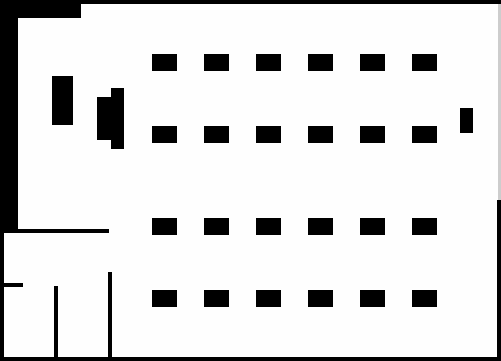
\includegraphics[width=\linewidth]{figures/cstam_map.png}
  \caption{Restaurant Lounge.}
\end{subfigure}
\caption{Occupancy-grid maps built with SLAM Toolbox.}
\label{fig:maps}
\end{figure}

\subsection{Navigation}

Navigation uses Nav2 with the NavFn global planner, the DWB local
controller and the default navigate-to-pose behaviour tree with its
recoveries. Each table has a waypoint in a YAML file
(\texttt{waypoints.yaml}, \texttt{resto\_arbi\_waypoints.yaml}): a service
point beside the table, facing it, so the robot never drives into chairs.
The task manager sends these poses through the \texttt{navigate\_to\_pose}
action.

\paragraph{Narrow doorways.} With default settings, Nav2's inflation layer
blocks Dar Tunibot's 1.20\,m doors, because the inflated zones of the two
door posts overlap. We kept the real robot radius and tuned the inflation
instead:
\[
  r_\text{robot}=0.28\,\text{m},\qquad r_\text{inflation}=0.42\,\text{m}\ (\text{from }0.55),\qquad k_\text{scale}=4.5
\]
\[
  W_\text{free} = W_\text{door} - 2\,r_\text{robot} = 1.20 - 0.56 = 0.64\,\text{m}.
\]
The steeper cost decay keeps the robot on the centreline of the doorway
while leaving a free corridor for the planner.

\begin{figure}[tbp]
\centering
\shot{0.9\linewidth}{rviz_nav.png}
\caption{Nav2 in RViz (Restaurant Lounge): the SLAM map with the global and local costmaps; the inflated zones around tables and walls keep the robot at a safe distance.}
\end{figure}

\subsection{Delivery task manager}

The task manager (\texttt{delivery\_task\_manager.py}) is the robot's
brain. It receives orders on \texttt{/delivery\_request}
(\texttt{\{"target": "Table 4", "item": "2x Thé à la menthe"\}}), gives
each one an id (\texttt{TASK-0001}, \ldots) and keeps a FIFO queue. When
the robot is free, it pops the next task and sends the Nav2 goal. On
arrival it waits at the table for the hand-over, marks the task completed
and pops the next one. Its state machine is shown in
Figure~\ref{fig:fsm}.

\begin{figure}[H]
\centering
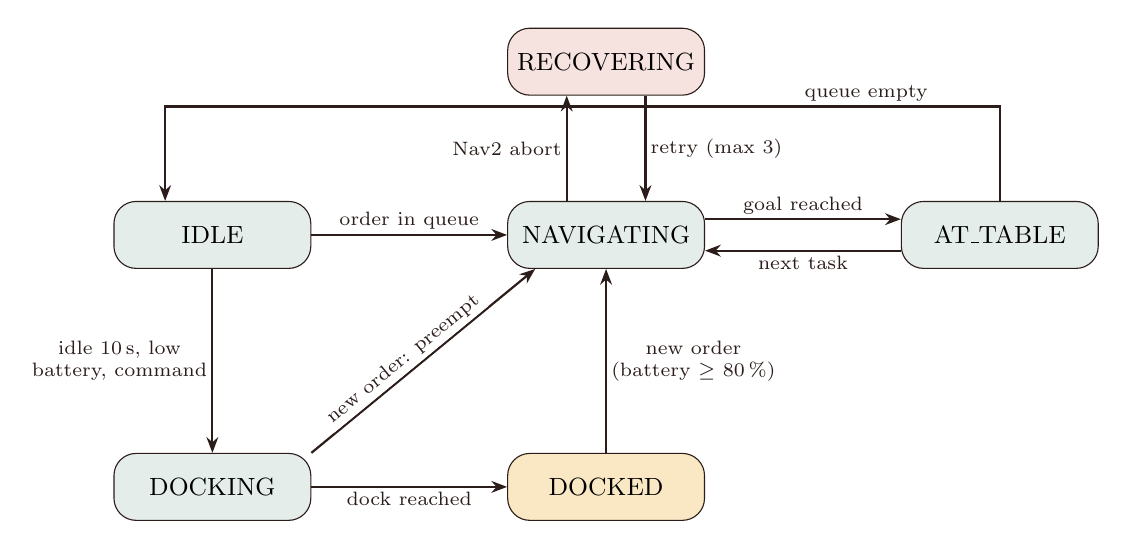
\begin{tikzpicture}[
  st/.style={draw=manganese,rounded corners=8pt,fill=copper!12,minimum width=2.5cm,minimum height=0.85cm,font=\small},
  arr/.style={-{Stealth[length=2mm]},thick,manganese},
  lab/.style={font=\scriptsize,fill=white,inner sep=1.5pt,align=center}
]
\node[st] (idle) at (0,0) {IDLE};
\node[st] (nav)  at (5,0) {NAVIGATING};
\node[st] (at)   at (10,0) {AT\_TABLE};
\node[st,fill=chili!15] (rec) at (5,2.2) {RECOVERING};
\node[st] (dk)   at (0,-3.2) {DOCKING};
\node[st,fill=ochre!30] (dd) at (5,-3.2) {DOCKED};
\draw[arr] (idle) -- node[lab,above]{order in queue} (nav);
\draw[arr] ([yshift=2mm]nav.east) -- node[lab,above]{goal reached} ([yshift=2mm]at.west);
\draw[arr] ([yshift=-2mm]at.west) -- node[lab,below]{next task} ([yshift=-2mm]nav.east);
\draw[arr] ([xshift=-5mm]nav.north) -- node[lab,left]{Nav2 abort} ([xshift=-5mm]rec.south);
\draw[arr] ([xshift=5mm]rec.south) -- node[lab,right]{retry (max 3)} ([xshift=5mm]nav.north);
\draw[arr] (at.north) -- ++(0,1.2) -| node[lab,pos=0.08,above]{queue empty} ([xshift=-6mm]idle.north);
\draw[arr] (idle) -- node[lab,left]{idle 10\,s, low\\battery, command} (dk);
\draw[arr] (dk) -- node[lab,below]{dock reached} (dd);
\draw[arr] (dd) -- node[lab,right]{new order\\(battery $\geq$ 80\,\%)} (nav);
\draw[arr] (dk.north east) -- node[lab,sloped,above,pos=0.45]{new order: preempt} ([xshift=-9mm]nav.south);
\end{tikzpicture}
\caption{Simplified state machine of the delivery task manager.}
\label{fig:fsm}
\end{figure}

\begin{itemize}
  \item \textbf{Live queue editing:} a pending task can be modified (table or item) or deleted through \texttt{/delivery\_task\_action}, without stopping the robot. An active task can be cancelled.
  \item \textbf{Preemption:} a new order that arrives while the robot is docking cancels the docking goal and is served at once (unless the battery is low).
  \item \textbf{Recovery:} when Nav2 aborts, the manager stops the robot, clears the costmaps, backs up ($v_x=-0.15$\,m/s for 1.8\,s) and re-plans, up to 3 times. If the table is still unreachable, the order goes back into the queue and the operator is alerted, so no order is lost.
  \item \textbf{Status:} the manager publishes \texttt{/robot\_system\_state} and a JSON \texttt{/delivery\_queue\_status} (current task, pending tasks, completed count, battery lock), which every interface reads.
\end{itemize}

\subsection{Auto-docking and battery}

\paragraph{Battery model.} \texttt{battery\_simulator.py} models a 24\,V
20\,Ah Li-ion NMC pack (7S, 480\,Wh). The open-circuit voltage follows a
non-linear curve between $V_\text{min}=21.0$\,V and $V_\text{max}=29.4$\,V:
\[
  V_\text{ocv}(s) = V_\text{min} + (V_\text{max}-V_\text{min})\left[0.84\,s + 0.16\,s^{0.3} - 0.05\,(1-s)^6\right]
\]
where $s$ is the state of charge. The load depends on motion,
$P = 35 + 65\,|v| + 30\,|\omega|$\,W (35\,W idle, about 130\,W when
cruising), and the terminal voltage sags under load through the internal
resistance, $V = V_\text{ocv} - I\,R_\text{int}$ with
$R_\text{int}=0.045\,\Omega$. Charge is counted in coulombs; charging
follows a CC--CV profile at 6\,A, and pack temperature is tracked. The node
publishes the standard \texttt{/battery\_state} and an extended JSON
\texttt{/battery\_status} at 1\,Hz.

\paragraph{Docking policy.} \texttt{docking\_controller.py} checks the
battery twice a second and decides when to go home:

\begin{table}[H]
\centering
\begin{tabularx}{\linewidth}{l l L}
\toprule
\textbf{State} & \textbf{Battery} & \textbf{Action} \\
\midrule
Normal & $> 25\,\%$ & Return to dock after 10\,s idle with an empty queue; a new order preempts it \\
Low & $\leq 25\,\%$ & Finish the current order, then \texttt{DOCK\_NOW:dock\_low\_battery}; no preemption \\
Critical & $\leq 15\,\%$ & Emergency \texttt{DOCK\_NOW:dock\_critical\_battery}, even during a delivery; the order stays queued \\
Charging & $< 80\,\%$ & Robot stays docked; new orders wait until 80\,\% \\
\bottomrule
\end{tabularx}
\caption{Return-to-dock policy.}
\end{table}

\begin{figure}[H]
\centering
\shot{0.32\linewidth}{gz_dock.png}
\caption{The robot parked and charging at its dock.}
\end{figure}

\subsection{Dynamic obstacle avoidance}

A pedestrian model walks through the restaurant, driven by
\texttt{dynamic\_obstacle\_controller.py} in four modes: \textsc{patrol}
(walks up and down an aisle at 0.35\,m/s), \textsc{cross} (crosses the
robot's path), \textsc{block} (steps into the path and stands still) and
\textsc{clear} (steps aside). The LiDAR sees the person, and the local
costmap, updated at 10\,Hz with 5\,m ray-tracing, marks the person and
clears the cells behind as they move. Nav2's controller and planner then
steer the robot around the person, or re-plan another route when the
aisle is blocked, and the delivery continues. The controller publishes
the pedestrian's position and mode on \texttt{/dynamic\_obstacle/status}
and RViz markers on \texttt{/dynamic\_obstacle/markers}.

\IfFileExists{figures/rviz_obstacle.png}{%
\begin{figure}[H]
\centering
\includegraphics[width=0.8\linewidth]{figures/rviz_obstacle.png}
\caption{The pedestrian on the robot's path: the local costmap marks the person and Nav2 plans around it.}
\end{figure}}{}

\subsection{Web interface (Phase 3)}

\begin{itemize}
  \item \texttt{ros\_bridge.py}: one ROS~2 node that subscribes to the robot topics and publishes the web commands.
  \item \texttt{store.py}: a thread-safe telemetry store that mirrors what the robot publishes and derives each web order's status.
  \item \texttt{server.py}: FastAPI REST endpoints, plus a WebSocket that pushes a full snapshot twice a second.
  \item \texttt{voice.py}: the voice-order parser (plain Python, no ROS).
  \item \texttt{static/}: Client and Admin pages in plain HTML, CSS and JavaScript, with no build step. Dish illustrations and icons are inline SVG, and the floor map is drawn on a canvas from the world file.
  \item \texttt{mock.py}: a simulated robot that reuses the real task queue and battery classes, for demos without Gazebo (\texttt{-{}-mock}).
\end{itemize}

\paragraph{Order tracking without changing the task manager.} The task
manager knows nothing about web orders. The bridge links an order to its
task by watching the queue status: the first new task id for the same
table with the same item text is that order. From then on its status
follows the task: queued, en route, at the table. When it leaves the
queue, a rise in the completed count means delivered; otherwise it is
reported as failed or cancelled. An order not picked up within 8\,s is
shown as not accepted. Each order is tracked on its own, so a guest can
follow several at once, and they are kept in the browser so tracking
resumes after a reload.

\paragraph{Voice ordering.} The client page can also take a spoken order; this bonus feature is described in Section~\ref{sec:bonus}.

\subsection{ROS 2 interface}

\begin{table}[H]
\centering
\small
\begin{tabularx}{\linewidth}{l l L}
\toprule
\textbf{Topic / action} & \textbf{From $\rightarrow$ to} & \textbf{Content} \\
\midrule
\texttt{/delivery\_request} & UI $\rightarrow$ task manager & new order (JSON: target, item) \\
\texttt{/delivery\_task\_action} & UI $\rightarrow$ task manager & modify, delete or cancel a task (JSON) \\
\texttt{/dock\_command} & controller / UI $\rightarrow$ task manager & \texttt{DOCK\_NOW:<reason>} or stop docking \\
\texttt{/dock\_state} & task manager $\rightarrow$ all & docked or not (Bool) \\
\texttt{/delivery\_queue\_status} & task manager $\rightarrow$ all & current task, pending tasks, completed count, battery lock (JSON) \\
\texttt{/robot\_system\_state} & task manager $\rightarrow$ all & IDLE, NAVIGATING, AT\_TABLE, RECOVERING, DOCKING, DOCKED \\
\texttt{navigate\_to\_pose} & task manager $\rightarrow$ Nav2 & action: goal pose of a table, kitchen or dock \\
\texttt{/cmd\_vel}, \texttt{/scan}, \texttt{/odom} & Nav2 $\leftrightarrow$ Gazebo & velocity commands, LiDAR, odometry \\
\texttt{/amcl\_pose}, \texttt{/plan} & Nav2 $\rightarrow$ UI & robot pose and global path \\
\texttt{/battery\_state}, \texttt{/battery\_status} & battery $\rightarrow$ controller / UI & percentage, voltage, current, power, temperature, flags (1\,Hz) \\
\texttt{/dynamic\_obstacle/cmd\_vel}, \texttt{/odom} & controller $\leftrightarrow$ Gazebo & drive the pedestrian, read its pose \\
\texttt{/dynamic\_obstacle/status} & controller $\rightarrow$ UI & pedestrian position and mode (JSON) \\
\texttt{/delivery\_waypoints} & web bridge $\rightarrow$ UI & world name and table coordinates (latched) \\
\bottomrule
\end{tabularx}
\caption{Main ROS 2 topics and actions.}
\end{table}

% =====================================================================
\section{Mockups}

The screens below are the working interfaces, captured from the running
system. They are the final UI, not drawings.

\subsection{Mission Control simulator (Phases 1 and 2)}

During Phases~1 and~2, we drove and tested the robot from a Mission
Control simulator written in Tkinter (\texttt{delivery\_simulator\_ui.py},
also available as a command-line tool for SSH sessions). It dispatches
orders with menu presets, shows the live queue with edit and delete,
controls docking, sets the battery to low or critical, and switches the
pedestrian's mode.

\begin{figure}[H]
\centering
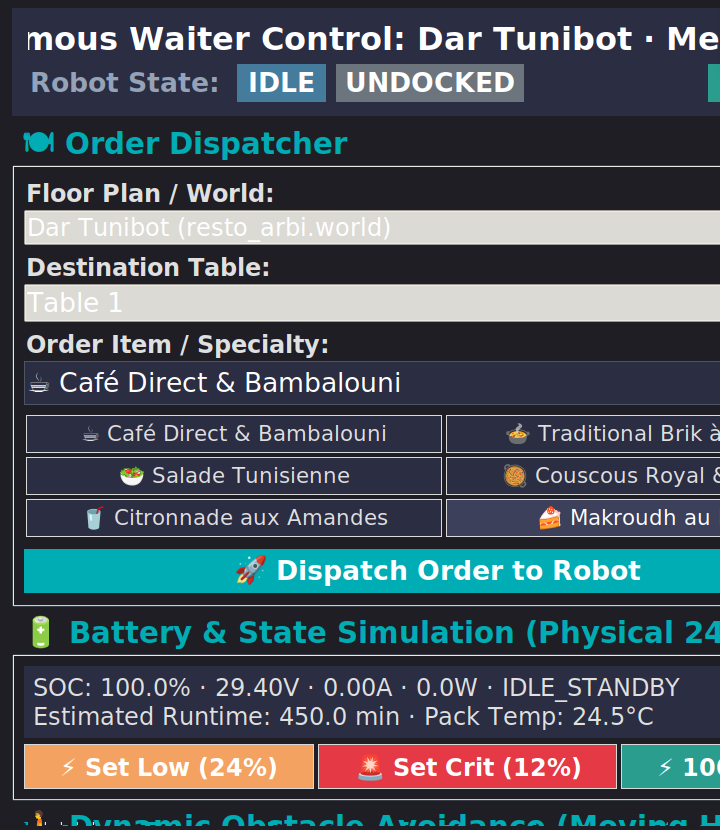
\includegraphics[width=0.55\linewidth]{figures/mission_control.png}
\caption{Mission Control simulator: order dispatcher and battery panel (Dar Tunibot).}
\end{figure}

\subsection{Design direction (Phase 3)}

For guests and staff we wanted an interface that feels like it belongs in
a Tunisian restaurant rather than a generic dashboard. The visual identity
borrows from Nabeul pottery: copper green, ochre and manganese brown on a
pale slip background. Headings use Bricolage Grotesque and body text uses
Atkinson Hyperlegible, a typeface designed for readability. Each dish has
its own flat illustration (Figure~\ref{fig:dishes}), and the menu behaves
like a real menu book with page turns. Motion is used only where it
carries meaning (a dish flying to the tray, the robot driving on the map)
and is turned off for users who ask for reduced motion.

\begin{figure}[H]
\centering
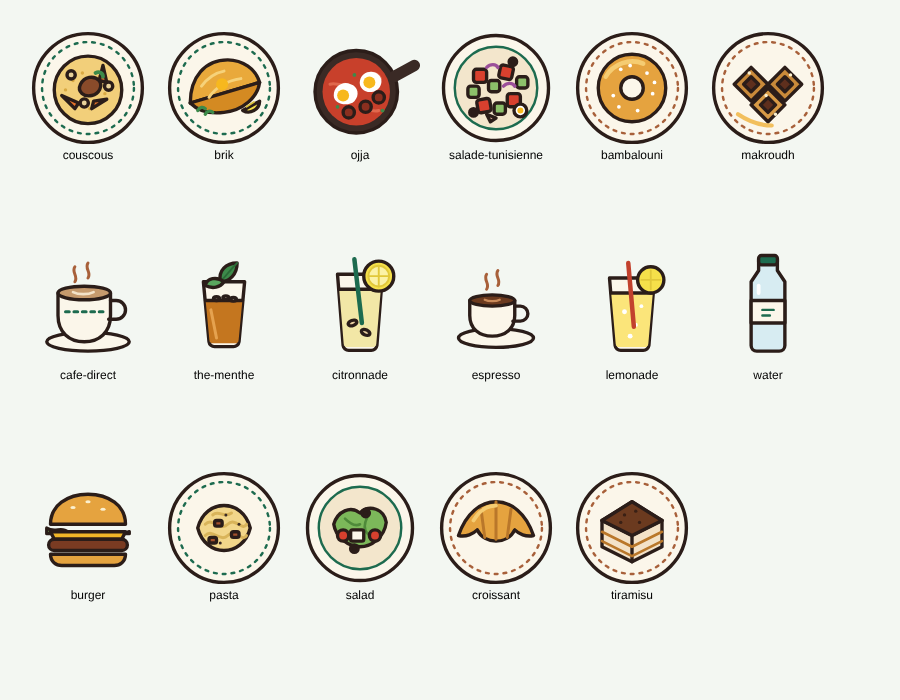
\includegraphics[width=0.5\linewidth]{figures/dishes.png}
\caption{Dish illustrations drawn for the Tunisian menu.}
\label{fig:dishes}
\end{figure}

\subsection{Client page}

The guest orders in three taps: table, dishes, Order. Everything else on
the page answers the guest's next question: is the robot free, where is my
order, when will it arrive.

\begin{figure}[H]
\centering
\begin{subfigure}[t]{0.24\linewidth}
  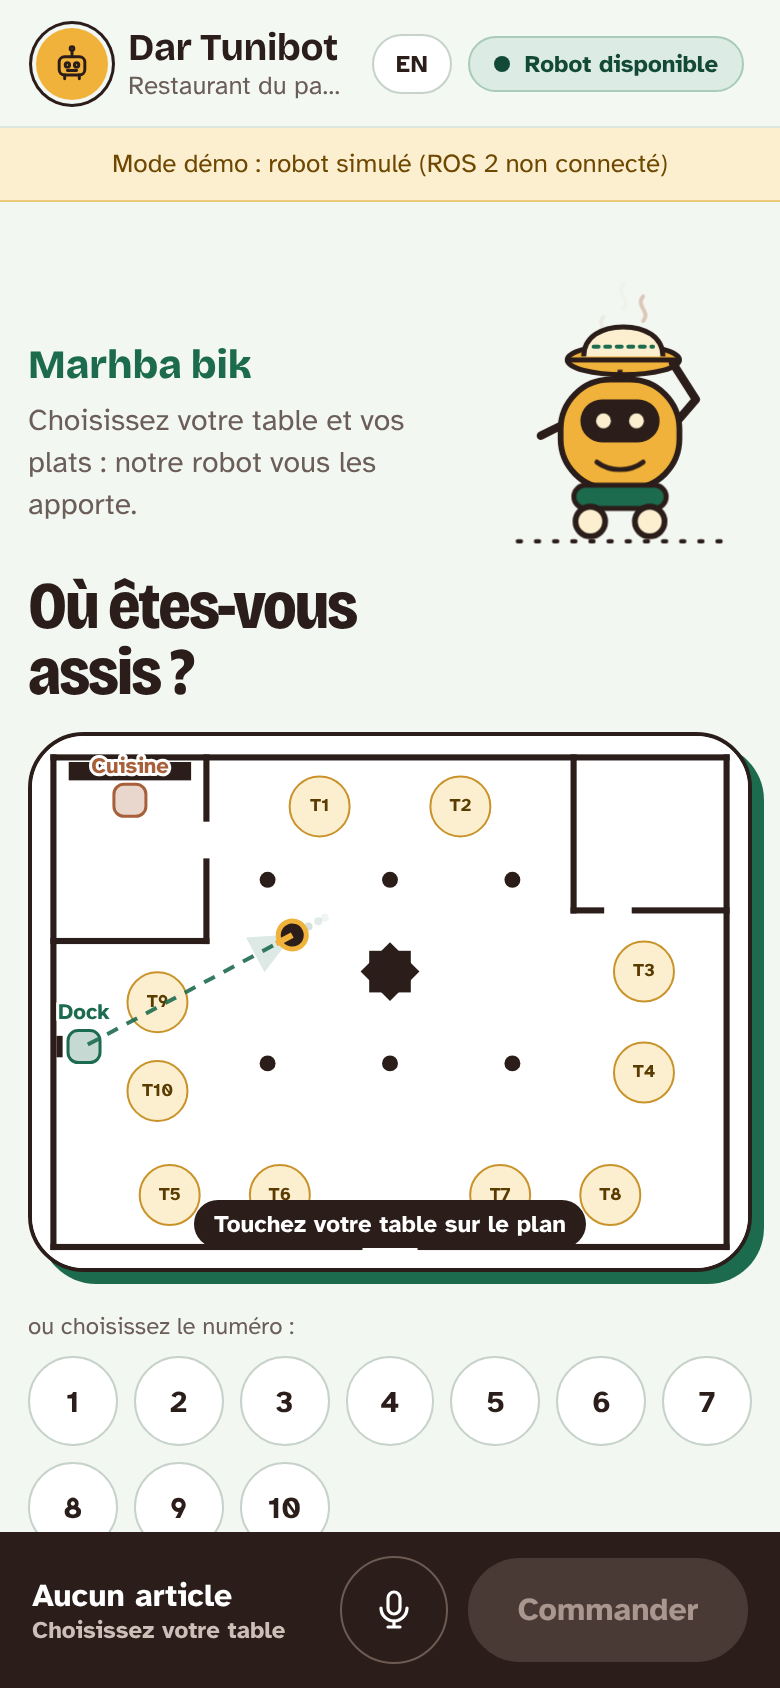
\includegraphics[width=\linewidth]{figures/client_table.png}
  \caption{Pick the table on the floor plan.}
\end{subfigure}\hfill
\begin{subfigure}[t]{0.24\linewidth}
  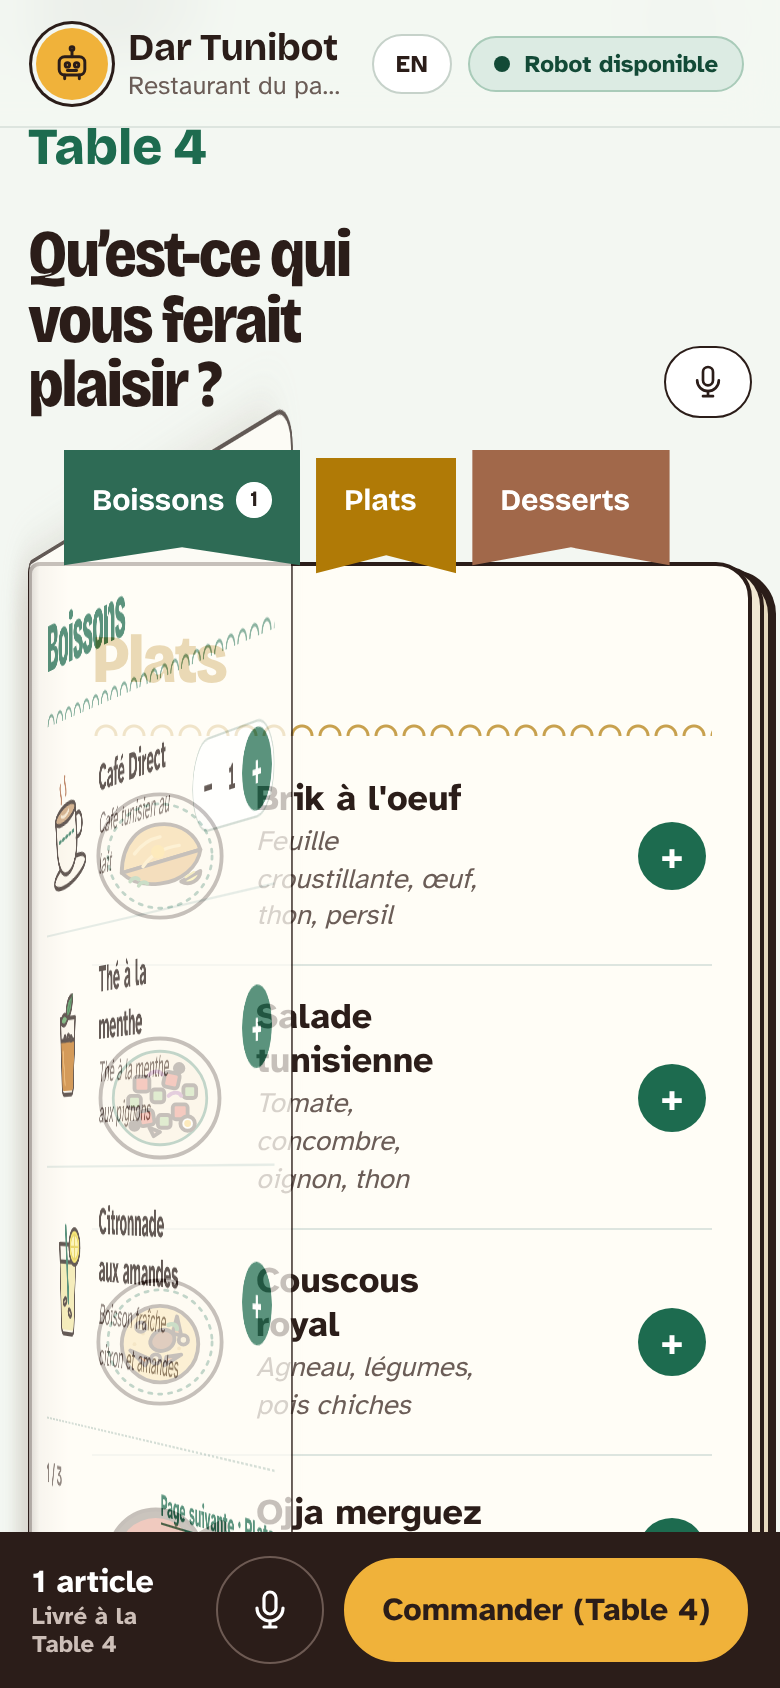
\includegraphics[width=\linewidth]{figures/client_menu.png}
  \caption{Menu book, one page per category.}
\end{subfigure}\hfill
\begin{subfigure}[t]{0.24\linewidth}
  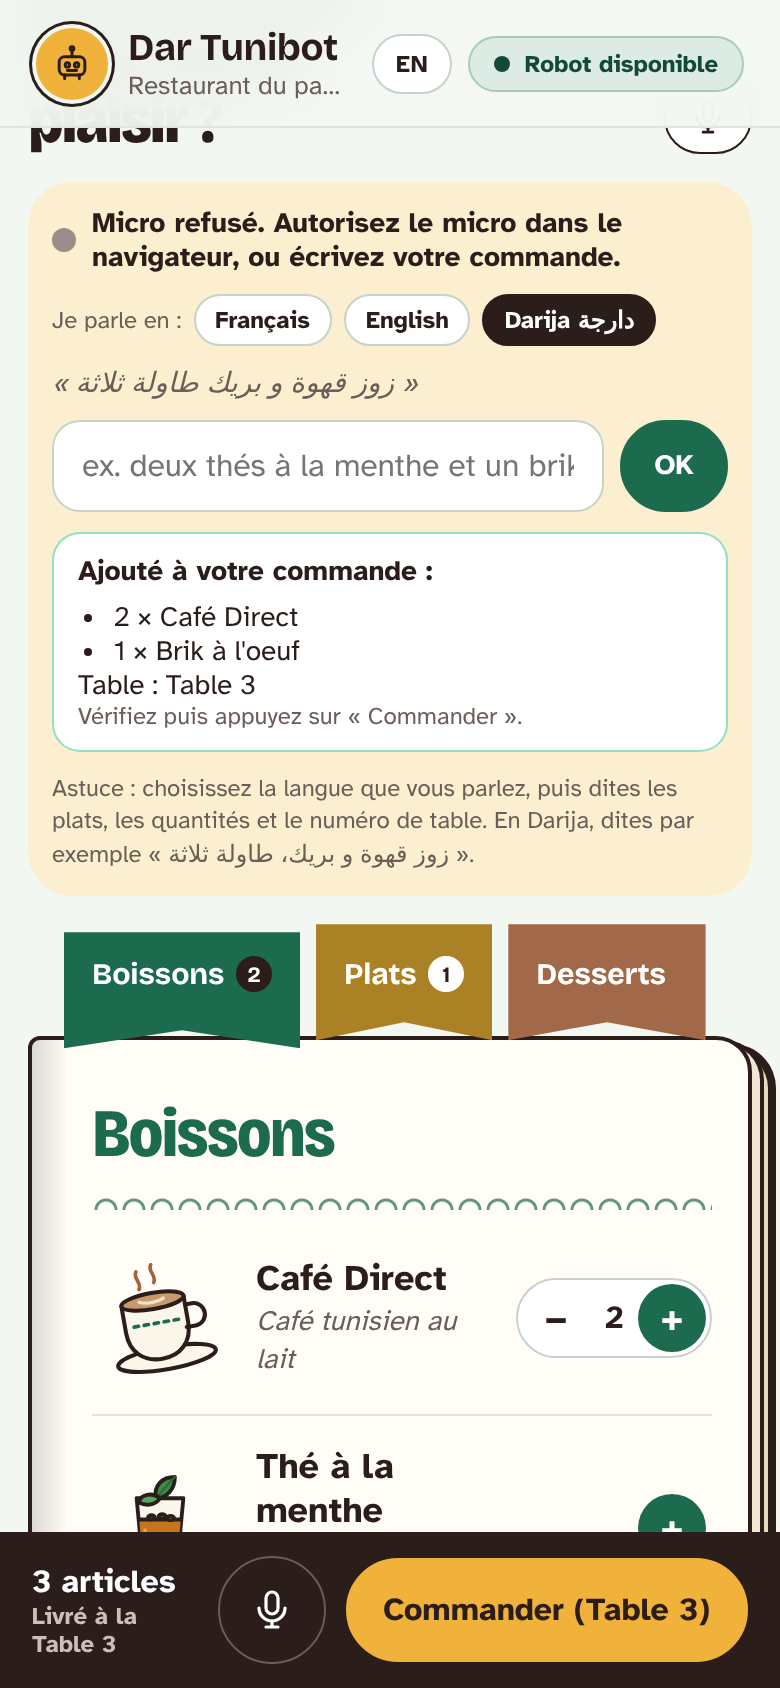
\includegraphics[width=\linewidth]{figures/client_voice.png}
  \caption{Voice order in Darija.}
\end{subfigure}\hfill
\begin{subfigure}[t]{0.24\linewidth}
  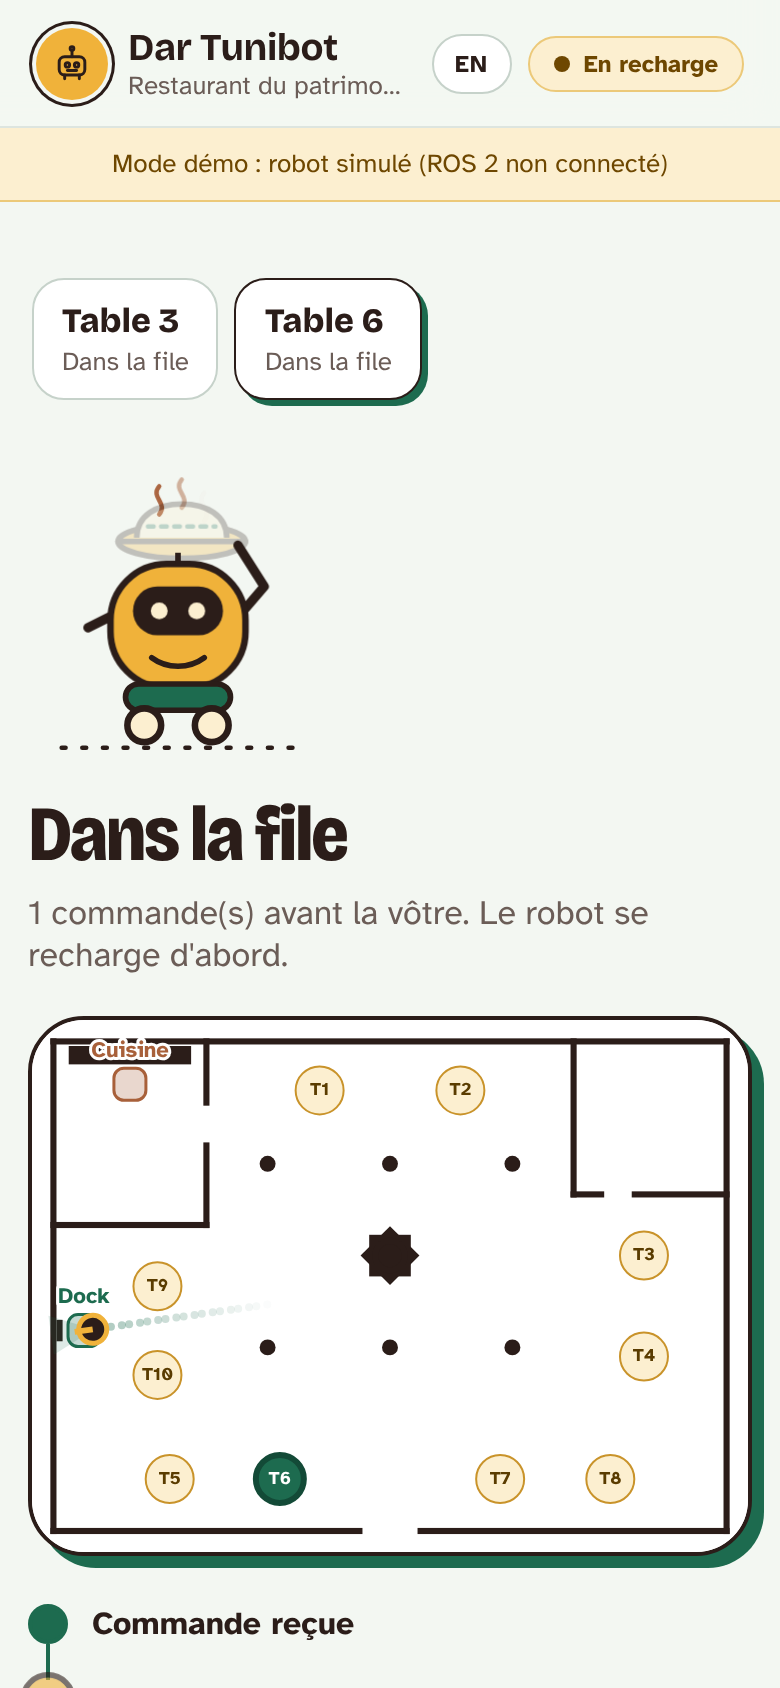
\includegraphics[width=\linewidth]{figures/client_orders.png}
  \caption{Several orders tracked at once.}
\end{subfigure}
\caption{Client page on a phone.}\label{fig:client}
\end{figure}

\begin{figure}[H]
\centering
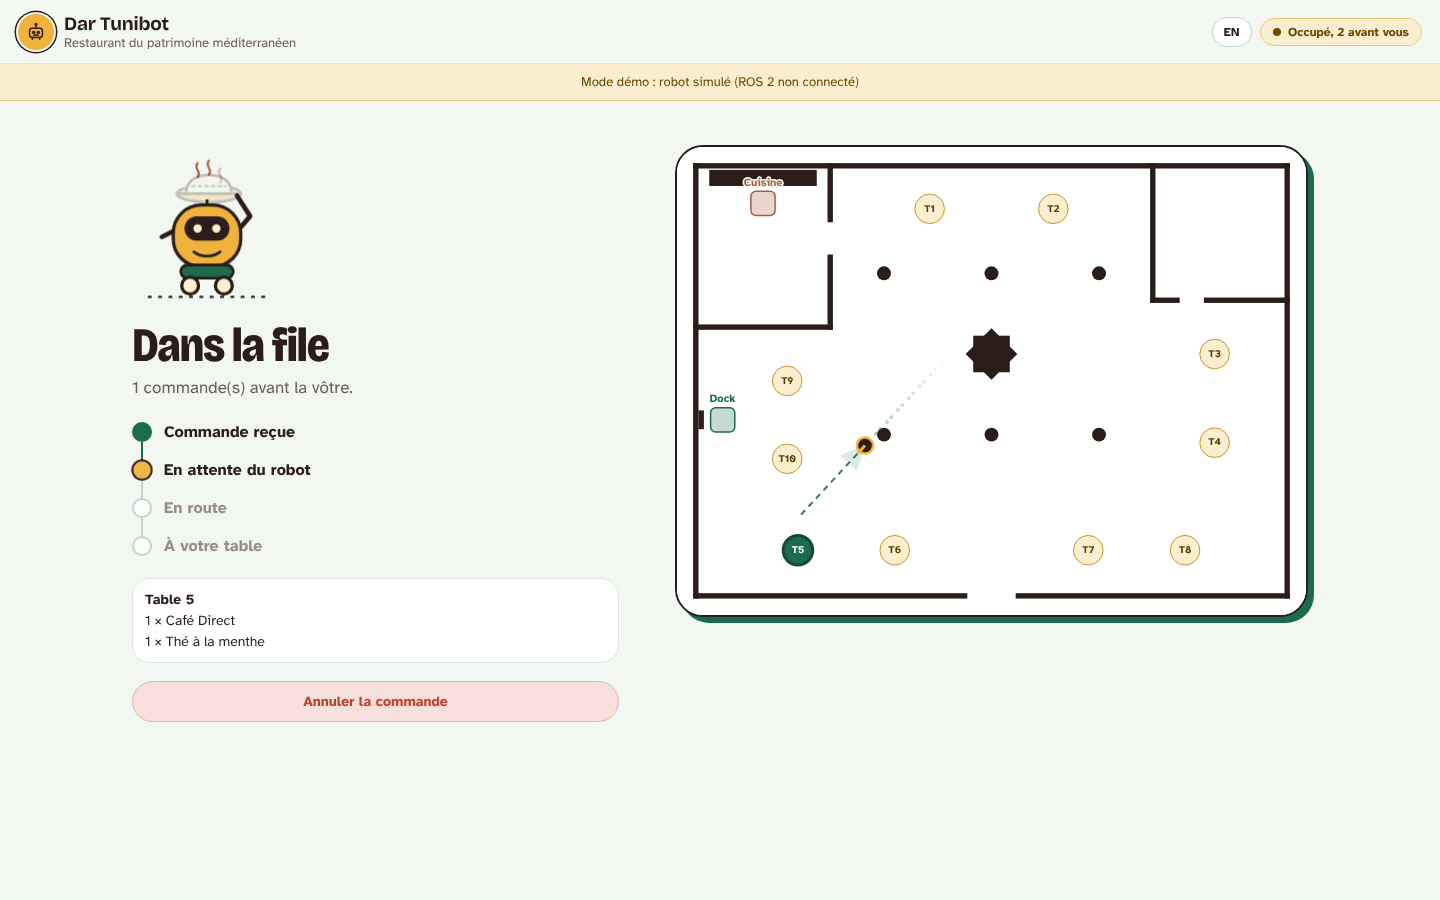
\includegraphics[width=0.85\linewidth]{figures/client_desktop.png}
\caption{Client page on a wide screen: the floor plan stays visible beside the order and the live tracking.}
\end{figure}

\paragraph{Edge cases handled.}
\begin{itemize}
  \item Robot offline (no battery heartbeat for 3\,s): red banner, ordering disabled.
  \item Battery lock (robot recharging to 80\,\%): order accepted; the guest is told it leaves after charging.
  \item Order not picked up by the task manager within 8\,s: ``not accepted, please ask the staff''.
  \item Navigation failure: ``a waiter will bring your order'' instead of a silent stop.
  \item Page reloaded or phone locked: orders are kept and tracking resumes.
  \item Lost Wi-Fi: the live connection reconnects on its own.
\end{itemize}

French is the default and English is one tap away; voice recognition has
its own language choice, because recognition must follow the language the
guest speaks, not the page language.

\subsection{Admin control room}

The Admin view at \texttt{/admin} shows, on one screen, everything staff
need to trust the robot: where it is, what it is doing, how much battery
it has left and what is waiting. The live floor map takes most of the
screen, a mission card floats over it, and the side column keeps every
panel open: orders, robot, battery, log and demo mode.

\begin{figure}[H]
\centering
\begin{subfigure}[t]{0.70\linewidth}
  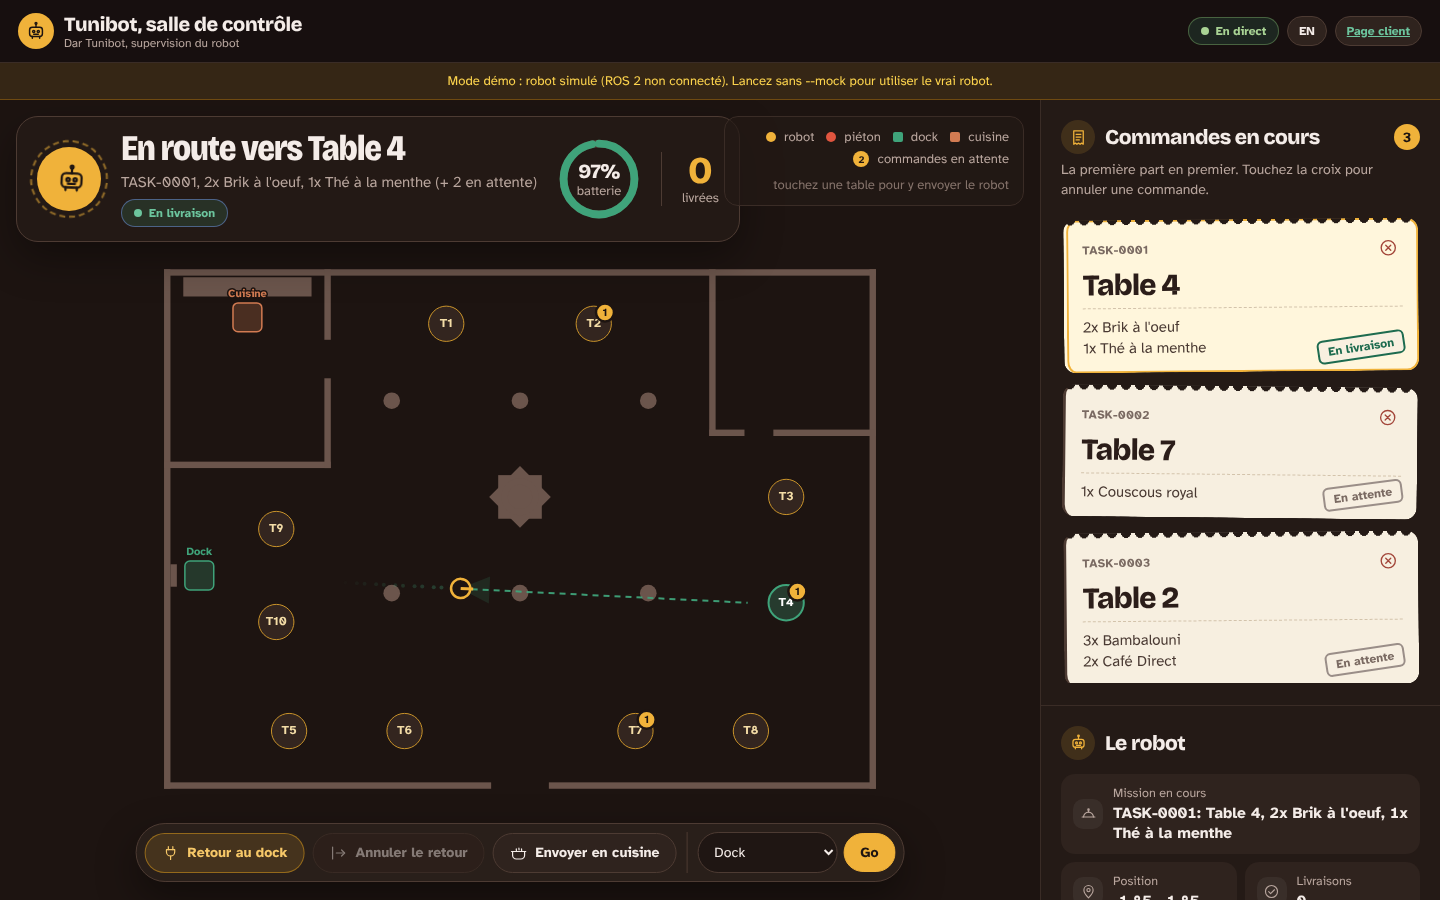
\includegraphics[width=\linewidth]{figures/admin_desktop.png}
  \caption{Live map with the Nav2 path, mission card and order tickets.}
\end{subfigure}\hfill
\begin{subfigure}[t]{0.25\linewidth}
  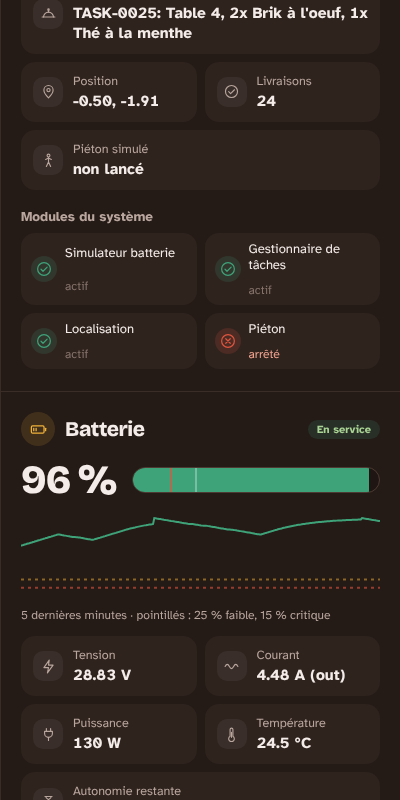
\includegraphics[width=\linewidth]{figures/admin_battery.png}
  \caption{Robot and battery panels.}
\end{subfigure}
\caption{Admin control room.}
\end{figure}

\begin{table}[H]
\centering
\small
\begin{tabularx}{\linewidth}{l L L}
\toprule
\textbf{Panel} & \textbf{Shows} & \textbf{Actions} \\
\midrule
Floor map & Walls, tables, dock and kitchen from the world file; robot pose, trail and Nav2 path; pedestrian; pending orders per table & Tap a table to send the robot there \\
Mission card & Current mission, state, battery ring, deliveries completed & -- \\
Orders & Current and pending orders as kitchen tickets & Cancel any order \\
Robot & Task, position, deliveries, pedestrian, health of each module & Return to dock, cancel the return, send to kitchen or a table \\
Battery & Percentage, voltage, current, power, temperature, runtime, 5-minute history & -- \\
Log & Last events: orders, state changes, battery warnings, voice orders & -- \\
Demo mode & -- & Battery 100\,\%, 24\,\% or 14\,\%; pedestrian patrol, cross, block or absent \\
\bottomrule
\end{tabularx}
\caption{Admin panels.}
\end{table}

% =====================================================================
\section{Bonus Functionalities}
\label{sec:bonus}

The bonus functionality we implemented is \textbf{voice command integration
for placing orders}. A guest can order by speaking, in French, English or
Tunisian Darija, instead of tapping through the menu. We also added several
extras beyond the required interface; they are listed in
Section~\ref{sec:extras}.

\subsection{Voice command integration for placing orders}

\paragraph{What the guest does.} On the Client page the guest taps the
microphone button, picks the spoken language (Français, English or Darija)
and says the whole order in one sentence, for example:
\begin{itemize}
  \item French: \emph{``deux thés à la menthe et un brik pour la table 4''}
  \item English: \emph{``two coffees and a couscous, table seven''}
  \item Darija: \emph{``zouz kahwa w brik, tawla tletha''} (two coffees and a brik, table three), also understood when the browser returns it in Arabic script.
\end{itemize}
The cart and the table fill in, the menu book opens on the page of the
first dish, and the page reads the order back aloud. The guest then
confirms with the Order button: nothing is sent to the robot before that
tap, so a misheard word can never send the robot to the wrong table.

\begin{figure}[H]
\centering
\resizebox{\linewidth}{!}{%
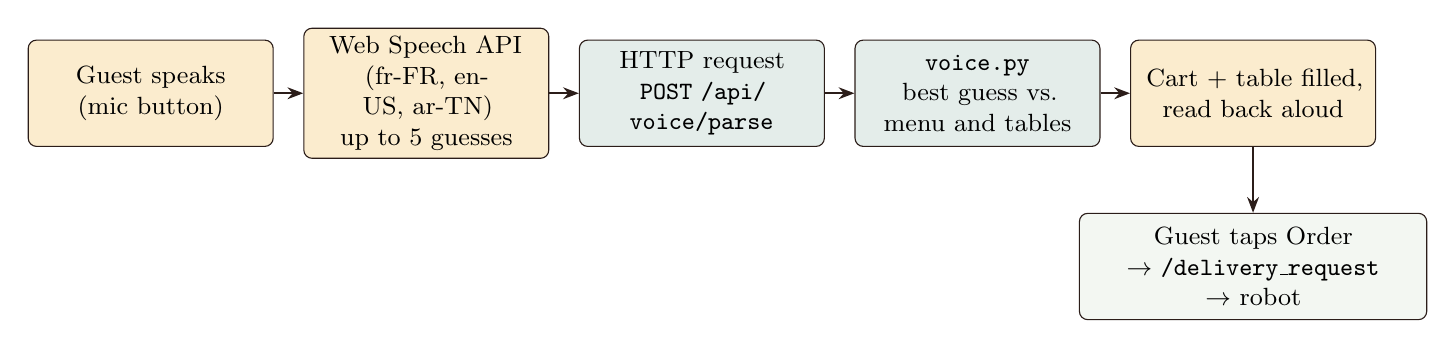
\begin{tikzpicture}[
  box/.style={draw=manganese,rounded corners=3pt,align=center,font=\small,
              minimum height=1.35cm,text width=2.9cm,inner sep=3pt},
  arr/.style={-{Stealth[length=2mm]},thick,manganese}
]
\node[box,fill=ochre!25] (mic) at (0,0) {Guest speaks\\(mic button)};
\node[box,fill=ochre!25] (asr) at (3.5,0) {Web Speech API\\(fr-FR, en-US, ar-TN)\\up to 5 guesses};
\node[box,fill=copper!12] (api) at (7.0,0) {HTTP request\\\texttt{POST /api/}\\\texttt{voice/parse}};
\node[box,fill=copper!12] (par) at (10.5,0) {\texttt{voice.py}\\best guess vs.\ menu and tables};
\node[box,fill=ochre!25] (cart) at (14.0,0) {Cart + table filled, read back aloud};
\node[box,fill=slip,text width=4.2cm] (ok) at (14.0,-2.2) {Guest taps Order\\$\rightarrow$ \texttt{/delivery\_request} $\rightarrow$ robot};
\draw[arr] (mic) -- (asr);
\draw[arr] (asr) -- (api);
\draw[arr] (api) -- (par);
\draw[arr] (par) -- (cart);
\draw[arr] (cart) -- (ok);
\end{tikzpicture}}
\caption{Voice ordering pipeline: the browser does speech-to-text, our parser turns the text into an order, the guest confirms.}
\end{figure}

\paragraph{How it works.}
\begin{enumerate}
  \item \textbf{Speech to text, in the browser.} Chrome or Edge turns the speech into text with the Web Speech API, in the language chosen in the voice panel (\texttt{fr-FR}, \texttt{en-US} or \texttt{ar-TN} for Darija). Listening continues through short pauses and stops after 2.5\,s of silence. The browser is asked for up to five alternative transcripts.
  \item \textbf{Parsing, on our server.} All alternatives go to \texttt{POST /api/voice/parse}. The parser \texttt{voice.py} (plain Python, no ROS, works offline) reads each one against the menu and the tables of the world that is running, and keeps the alternative that fits best: most dishes recognised, a table found, fewest unknown words.
  \item \textbf{Confirmation.} The page fills the cart and the table, shows what it understood (and any word it could not place), and speaks the order back with speech synthesis. The guest confirms or corrects it by hand.
\end{enumerate}

\paragraph{What the parser understands.}
\begin{table}[H]
\centering
\small
\begin{tabularx}{\linewidth}{l L}
\toprule
\textbf{Element} & \textbf{Examples} \\
\midrule
Quantities & French \emph{un, deux, trois}\ldots; English \emph{one, two, three}\ldots; Darija \emph{wahed, zouz, tletha, arba}\ldots; digits, including Arabic-Indic digits \\
Tables & \emph{table 4}, \emph{table numéro 10}, \emph{table seven}, \emph{tawla tletha}, Arabic \emph{taawila} with a number \\
Dish names and aliases & \emph{thé à la menthe / atay / tay}, \emph{café / kahwa}, \emph{couscous / kousksi} \\
Speech-to-text mistakes & \emph{brique} $\rightarrow$ brik, \emph{bamba louni} $\rightarrow$ bambalouni, \emph{makrout} $\rightarrow$ makroudh \\
Darija in Arabic script & known words mapped directly (numbers, \emph{table}, dish names, ``and''), the rest transliterated to Latin letters before matching \\
Filler words & \emph{je voudrais}, \emph{s'il vous plaît}, \emph{please}, \emph{n7eb}, \emph{aatini} are ignored \\
\bottomrule
\end{tabularx}
\caption{Language coverage of the voice parser.}
\end{table}

Matching combines accent folding, plural removal, a phonetic key and fuzzy
string matching. A dish that is not on the menu is reported to the guest,
never replaced by a guess, and a table that does not exist in the current
world is rejected. Quantities are capped at nine per dish, like on the
touch menu.

\paragraph{Design decision from testing.} The first version used the page
language for recognition. On an English page, French speech came back as
nonsense (``\ldots uventies and a birthday before''). The voice panel
therefore has its own language choice, and French is the default because
it is what most guests in Tunisia speak to a machine.

\paragraph{Testing.} 28 automated tests cover the parser: French, English
and Darija sentences in Latin and Arabic script, sound-alike spellings,
unknown dishes, tables that do not exist, the quantity cap and the choice
of the best alternative. Two browser end-to-end tests (Playwright) check
the full flow: a voice order is parsed, confirmed, sent to the simulated
robot and reaches ``Delivered'', and the microphone flow keeps the best of
several alternatives. Figure~\ref{fig:client}\,(c) shows a Darija order on
a phone.

\paragraph{Limits.} Speech recognition depends on the browser (Chrome or
Edge) and on its online service, and browsers only allow the microphone on
\texttt{localhost} or HTTPS. An on-device model is listed in the future
improvements.

\subsection{Additional features beyond the requirements}
\label{sec:extras}

\begin{table}[H]
\centering
\small
\begin{tabularx}{\linewidth}{l L}
\toprule
\textbf{Feature} & \textbf{What it adds} \\
\midrule
Several orders at once & A guest can place a new order while earlier ones are still on their way and follow each one separately; orders survive a page reload \\
Table picked on the floor plan & The guest taps their table on the real restaurant plan, and can watch the robot drive to it \\
Arrival estimate & Remaining Nav2 path length turned into a time estimate while the robot drives \\
Bilingual interface & Client and Admin pages in French and English, with translated dish descriptions \\
Illustrated menu book & Menu with page turns and a drawing for every dish, following the world that is running (Tunisian menu for Dar Tunibot) \\
Battery monitoring panel & Live percentage, voltage, current, power, temperature, runtime and a 5-minute history with the 25\,\% and 15\,\% thresholds \\
Live control room & Robot, Nav2 path, pedestrian and pending orders per table on one map; tap a table to send the robot \\
Demo mode & Buttons to set the battery to low or critical and to change the pedestrian's behaviour, to show the robot's reactions live \\
Mock robot & The whole interface runs without ROS or Gazebo (\texttt{-{}-mock}), reusing the real queue and battery classes, for demos and tests \\
\bottomrule
\end{tabularx}
\caption{Additional features.}
\end{table}

% =====================================================================
\section{Technologies, Frameworks and Tools}

\begin{table}[H]
\centering
\begin{tabularx}{\linewidth}{l l L}
\toprule
\textbf{Area} & \textbf{Technology} & \textbf{Use} \\
\midrule
Middleware & ROS~2 Jazzy & Nodes, topics, actions, launch files, colcon build \\
Simulation & Gazebo Harmonic, ros\_gz & Restaurant worlds, BellaBot, LiDAR, pedestrian, bridge to ROS~2 \\
Navigation & Nav2 (NavFn, DWB) & Path planning, control, behaviour tree, recoveries \\
Mapping / localization & SLAM Toolbox, AMCL & Building the maps, localizing on them \\
Visualisation & RViz~2 & Map, costmaps, paths and markers \\
Robot logic & Python 3.12 (rclpy) & Task manager, docking, battery, pedestrian controller \\
Operator tool & Tkinter & Mission Control simulator (GUI and CLI) \\
Web server & FastAPI, Uvicorn, Pydantic & REST API, WebSocket, request validation \\
Front end & HTML5, CSS3, JavaScript & Client and Admin pages (no framework), canvas map, SVG illustrations \\
Speech (bonus) & Web Speech API & Speech recognition and read-back in the browser \\
Testing & pytest, unittest, Playwright & Unit, integration and browser end-to-end tests \\
Tools & Git, GitHub, VS Code & Version control, pull requests, development on Ubuntu 24.04 \\
\bottomrule
\end{tabularx}
\caption{Technologies used.}
\end{table}

% =====================================================================
\section{Development Milestones}

\begin{table}[H]
\centering
\small
\begin{tabularx}{\linewidth}{l L}
\toprule
\textbf{Milestone} & \textbf{Delivered} \\
\midrule
Phase 1.1 -- Simulation & Restaurant Lounge world, BellaBot model with LiDAR and odometry, Gazebo--ROS bridge \\
Phase 1.2 -- Mapping and navigation & SLAM map, AMCL localization at the dock, Nav2 configuration, 24 table waypoints \\
Phase 1.3 -- Delivery logic & Task queue manager with edit, delete and preemption; auto-docking; Mission Control simulator; 9 unit tests \\
\midrule
Phase 2.1 -- Dynamic obstacles & Pedestrian model and controller (4 modes), 10\,Hz local costmap, RViz markers \\
Phase 2.2 -- Complex layouts & Dar Tunibot world and map, inflation tuning for 1.20\,m doorways, multi-stage recovery \\
Phase 2.3 -- Battery & Physical Li-ion model, low / critical / recharge docking policy; 5 integration tests and test report \\
\midrule
Phase 3.1 -- Web interface & \texttt{cstam\_web} package: Client and Admin pages, ROS~2 bridge, mock mode; web order delivered in Gazebo \\
Phase 3.2 -- UX and voice & Voice orders (French, English, Darija), arrival estimate, order review, edge cases, automated tests \\
Phase 3.3 -- Design & Nabeul pottery identity, dish illustrations, menu book, table on the floor plan, several orders, Admin control room \\
Phase 3.4 -- Documentation & This report, README and demonstration video \\
\bottomrule
\end{tabularx}
\caption{Development milestones.}
\end{table}

% =====================================================================
\section{Testing Results}

\subsection{Automated tests}

\begin{table}[H]
\centering
\small
\begin{tabularx}{\linewidth}{l c c L}
\toprule
\textbf{Suite} & \textbf{Phase} & \textbf{Tests} & \textbf{What it checks} \\
\midrule
\texttt{test\_system.py} & 1 & 9 & Workspace files, 26 waypoints, queue lifecycle (queued $\rightarrow$ en route $\rightarrow$ completed), modify and delete, auto-docking idle trigger \\
\texttt{test\_system\_phase2.py} & 2 & 5 & Obstacle detection, doorway clearance, corridor recovery, battery physics, low and critical docking triggers \\
\texttt{cstam\_web/test\_web.py} & 3 & 16 & Order lifecycle follows the task manager, order matching, cancelled / rejected / failed orders, offline detection, battery lock, validation, admin commands, WebSocket \\
\texttt{cstam\_web/test\_voice.py} & 3 & 28 & French, English and Darija sentences, sound-alike spellings, unknown dish reported, table must exist, best alternative kept \\
\texttt{cstam\_web/test\_e2e\_browser.py} & 3 & 7 & Voice order delivered end to end, microphone flow, table on the floor plan, menu book, languages, admin map click, several orders \\
\midrule
\textbf{Total} & & \textbf{65} & \textbf{All passing} \\
\bottomrule
\end{tabularx}
\caption{Automated test suites (parametrised cases counted individually).}
\end{table}

\subsection{Phase 2 test cases}

\begin{table}[H]
\centering
\small
\begin{tabularx}{\linewidth}{l L L}
\toprule
\textbf{Test case} & \textbf{Input} & \textbf{Result} \\
\midrule
TC-01 Obstacle detection & Pedestrian 1.0\,m ahead, walking at 0.35\,m/s & Detected, local costmap marked, robot avoids contact \\
TC-02 Doorway clearance & 1.20\,m door, $r_\text{robot}=0.28$, $r_\text{infl}=0.42$, $k=4.5$ & Free corridor 0.64\,m, path found through the door \\
TC-03 Corridor recovery & Nav2 abort in a corridor & Reverse 1.8\,s at $-0.15$\,m/s, costmap cleared, order kept \\
TC-04 Battery physics & Discharge 100\,\% $\rightarrow$ 20\,\% & 29.4\,V $\rightarrow$ 21.8\,V, 0.29\,V sag at 130\,W \\
TC-05 Docking triggers & SoC 24.9\,\% and 14.9\,\% & Low and critical dock commands within 15\,ms \\
\bottomrule
\end{tabularx}
\caption{Phase 2 test cases (all passed).}
\end{table}

\subsection{Scenario tests in Gazebo}

\begin{table}[H]
\centering
\small
\begin{tabularx}{\linewidth}{l L c}
\toprule
\textbf{Scenario} & \textbf{Observed} & \textbf{Result} \\
\midrule
Deliveries to all 24 tables (Lounge) & Smooth paths through every aisle, no collision & Pass \\
Deliveries through 1.20\,m arches (Dar Tunibot) & Robot passes on the doorway centreline & Pass \\
Edit and delete a queued order & Queue updated live, active delivery not disturbed & Pass \\
Return to dock, then stop docking & Robot drives to the dock; stops and goes IDLE on command & Pass \\
New order during docking & Docking cancelled, robot turns to the table & Pass \\
Pedestrian crossing or blocking the aisle & Robot steers around or re-plans, delivery continues & Pass \\
Battery set to 24\,\% / 14\,\% & Home after the queue / emergency return at once & Pass \\
Order from the web Client page & \texttt{TASK-0003} delivered to Table~4; page shows on the way, at your table, delivered & Pass \\
\bottomrule
\end{tabularx}
\caption{End-to-end scenarios run in Gazebo.}
\end{table}

\subsection{Issues found and fixed}
\label{sec:issues}

\begin{itemize}
  \item \textbf{Floating pedestrian.} The first pedestrian model had no gravity and a single link; contact with chairs tipped it 90° and it floated through the room. We rebuilt it on a hidden differential-drive chassis with gravity, a low centre of mass and casters, and drove it with a heading-and-speed controller. It now stays upright and visible to the LiDAR.
  \item \textbf{Robot not going home on critical battery.} The task manager assumed the robot was at the dock because its last pose defaulted to the dock coordinates, so it never sent the Nav2 goal. Using the latest AMCL pose fixed it.
  \item \textbf{Blocked doorways.} Default inflation closed Dar Tunibot's doors; fixed by the tuning in Section~4.4.
  \item \textbf{Voice language.} On an English page, French speech came back as nonsense; the voice panel got its own language choice.
\end{itemize}

% =====================================================================
\section{Future Improvements}

\begin{itemize}
  \item \textbf{Real robot:} run the same stack on a physical base; the web layer needs no change since it only uses ROS~2 topics.
  \item \textbf{People-aware navigation:} predict pedestrian motion (social costmap layers) instead of treating people as obstacles that appear.
  \item \textbf{Fleet:} several robots on one Admin map, with orders assigned to the nearest free robot.
  \item \textbf{Batched deliveries:} serve several tables on one trip using the robot's trays.
  \item \textbf{Kitchen screen:} a page for the kitchen to mark an order ready before the robot leaves.
  \item \textbf{Offline speech:} an on-device speech model (e.g.\ Whisper) for voice ordering without a cloud service and with better Darija accuracy.
  \item \textbf{Security and analytics:} HTTPS and staff login for the Admin page; delivery times, battery cycles and busiest tables over a day.
\end{itemize}

% =====================================================================
\section*{References}
\addcontentsline{toc}{section}{References}

\begin{enumerate}[label={[\arabic*]}]
  \item S.~Macenski, T.~Foote, B.~Gerkey, C.~Lalancette, W.~Woodall, ``Robot Operating System 2: Design, architecture, and uses in the wild,'' \emph{Science Robotics}, vol.~7, no.~66, 2022.
  \item S.~Macenski, F.~Martín, R.~White, J.~Ginés Clavero, ``The Marathon 2: A Navigation System,'' \emph{IEEE/RSJ IROS}, 2020.
  \item S.~Macenski, I.~Jambrecic, ``SLAM Toolbox: SLAM for the dynamic world,'' \emph{Journal of Open Source Software}, vol.~6, no.~61, 2021.
  \item S.~Thrun, W.~Burgard, D.~Fox, \emph{Probabilistic Robotics}. MIT Press, 2005.
  \item D.~Fox, W.~Burgard, S.~Thrun, ``The dynamic window approach to collision avoidance,'' \emph{IEEE Robotics \& Automation Magazine}, vol.~4, no.~1, 1997.
  \item Open Robotics, ``ROS~2 Jazzy documentation,'' \url{https://docs.ros.org/en/jazzy/}.
  \item Open Robotics, ``Gazebo Harmonic documentation,'' \url{https://gazebosim.org/docs/harmonic}.
  \item Nav2 project, ``Nav2 documentation,'' \url{https://docs.nav2.org/}.
  \item S.~Ramírez, ``FastAPI,'' \url{https://fastapi.tiangolo.com/}.
  \item W3C Community Group, ``Web Speech API,'' \url{https://webaudio.github.io/web-speech-api/}.
  \item Microsoft, ``Playwright for Python,'' \url{https://playwright.dev/python/}.
  \item W3C, ``Web Content Accessibility Guidelines (WCAG) 2.1,'' 2018.
\end{enumerate}

\end{document}
